% Expert-audience Beamer deck: encoding effort + BMC-vs-ITP positioning.
% Compile:  pdflatex poc-status-expert-beamer.tex   (run twice)
\documentclass[aspectratio=169,11pt]{beamer}

\usetheme{Madrid}
\usepackage{tikz}
\usetikzlibrary{arrows.meta,positioning}
\usepackage{booktabs}
\usepackage{xcolor}
\usepackage{pifont}

\definecolor{accent}{HTML}{0B5CAD}
\definecolor{warn}{HTML}{B3261E}
\definecolor{ok}{HTML}{1A7F37}
\definecolor{panel}{HTML}{EEF2F7}

\setbeamercolor{structure}{fg=accent}
\setbeamercolor{frametitle}{bg=accent,fg=white}
\setbeamercolor{title}{bg=accent,fg=white}
\setbeamertemplate{navigation symbols}{}
\setbeamertemplate{itemize items}[circle]
\setbeamerfont{frametitle}{size=\large}

\newcommand{\good}{\textcolor{ok}{\ding{51}}}
\newcommand{\bad}{\textcolor{warn}{\ding{55}}}

\title[PyTorch $\equiv$ checking with ESBMC]{Formal equivalence checking of PyTorch programs with ESBMC}
\subtitle{BMC for fusion/rewrite correctness --- and how the encoding compares to interactive proof}
\date{Proof-of-concept $\cdot$ status update (expert version)}
\author{Lucas Cordeiro}
\institute{University of Manchester}

\begin{document}

{\setbeamertemplate{footline}{}
\begin{frame}[plain]
  \centering\vfill
  \begin{beamercolorbox}[sep=14pt,center,rounded=true,shadow=true,wd=0.92\textwidth]{title}
    \usebeamerfont{title}\inserttitle
  \end{beamercolorbox}
  \vskip0.7em
  {\small\textcolor{accent}{\insertsubtitle}}\par
  \vskip1.4em
  {\large\insertauthor}\par\smallskip
  {\small\insertinstitute}\par\vskip1em
  {\insertdate}\vfill
\end{frame}}

% ---------------------------------------------------------------
\begin{frame}{Problem \& threat model}
  Optimising transformations --- \textbf{operator fusion, kernel rewrites, compiler passes} ---
  must be semantics-preserving. We decide:
  \[ \forall\, X, W \text{ with entries in } [-10,10].\quad P_{\text{unfused}}(X,W)\ \equiv\ P_{\text{fused}}(X,W) \]
  \begin{itemize}
    \item \textbf{Testing} under-approximates: it samples a finite input set.
    \item We want \textbf{exhaustive} equivalence over an input region, with
      \textbf{bit-precise IEEE-754} (where fusion breaks: reassociation, rounding).
    \item Two verdicts: \textbf{proof} (UNSAT) or a \textbf{concrete counterexample} (SAT).
  \end{itemize}
  \medskip
  {\footnotesize Checked under a \textbf{sequential IEEE-754 semantics}; inputs are bounded, so
  \textbf{NaN/Inf are excluded} --- equivalence is proven over finite FP domains.
  \textbf{Not modelled:} backend optimisations (FMA, cuBLAS), parallel/tree reductions, scheduling.}
\end{frame}

% ---------------------------------------------------------------
\begin{frame}{Running example: QKV projection}
  \[
    \text{unfused: } Q = XW_q,\; K = XW_k,\; V = XW_v
  \]
  \[
    \text{fused: } W = [\,W_q \mid W_k \mid W_v\,],\quad \mathit{QKV}=XW,\quad \text{split}
  \]

  \bigskip
  The fused column $j$ is the \textbf{identical multiply--add sequence} as the corresponding
  unfused projection $\Rightarrow$ the two are equal \textbf{bit-for-bit under the same
  evaluation order} (sequential IEEE-754), not merely within a tolerance. Both claims are checked.
\end{frame}

% ---------------------------------------------------------------
\begin{frame}{The two programs, side by side}
  \centering
  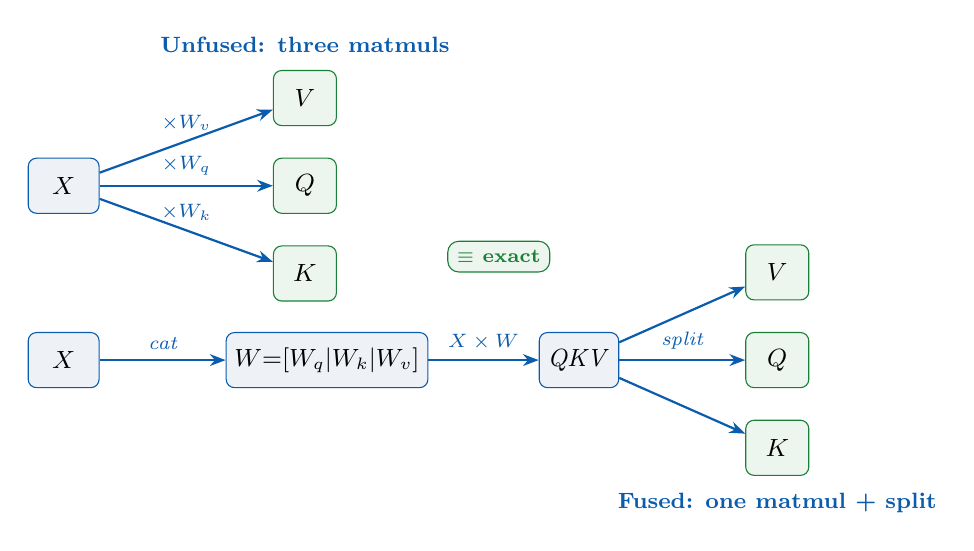
\begin{tikzpicture}[
      font=\small,
      box/.style={rounded corners=3pt,draw=accent,fill=panel,minimum height=7mm,minimum width=9mm,inner sep=3pt},
      res/.style={rounded corners=3pt,draw=ok,fill=ok!8,minimum height=7mm,minimum width=8mm},
      op/.style={midway,above,font=\scriptsize\itshape,text=accent},
      arr/.style={-{Stealth[length=2mm]},thick,accent}]
    \node[box] (xu) {$X$};
    \node[res,right=22mm of xu] (Q) {$Q$};
    \node[res,below=4mm of Q] (K) {$K$};
    \node[res,above=4mm of Q] (V) {$V$};
    \draw[arr] (xu) -- (V) node[op]{$\times W_v$};
    \draw[arr] (xu) -- (Q) node[op]{$\times W_q$};
    \draw[arr] (xu) -- (K) node[op]{$\times W_k$};
    \node[above=1mm of V,text=accent,font=\footnotesize\bfseries] {Unfused: three matmuls};
    \node[box,below=15mm of xu] (xf) {$X$};
    \node[box,right=16mm of xf] (W) {$W{=}[W_q|W_k|W_v]$};
    \node[box,right=14mm of W] (QKV) {$\mathit{QKV}$};
    \node[res,right=16mm of QKV] (Qf) {$Q$};
    \node[res,below=4mm of Qf] (Kf) {$K$};
    \node[res,above=4mm of Qf] (Vf) {$V$};
    \draw[arr] (xf) -- (W) node[op]{cat};
    \draw[arr] (W) -- (QKV) node[op]{$X\times W$};
    \draw[arr] (QKV) -- (Vf) node[op,font=\tiny\itshape]{};
    \draw[arr] (QKV) -- (Qf) node[op]{split};
    \draw[arr] (QKV) -- (Kf) node[op,font=\tiny\itshape]{};
    \node[below=1mm of Kf,text=accent,font=\footnotesize\bfseries] {Fused: one matmul {+} split};
    \node[draw=ok,rounded corners,fill=ok!8,text=ok,font=\scriptsize\bfseries,
          right=14mm of Q,yshift=-9mm,align=center] {$\equiv$ exact};
  \end{tikzpicture}
\end{frame}

% ---------------------------------------------------------------
\begin{frame}{The embedding (1/2): encoding design}
  The program \textbf{acts as the specification} under the assumed operational model
  (correctness depends on the OM's faithfulness) --- no separate spec to maintain.
  \begin{itemize}
    \item \textbf{Tensors} $\to$ nested lists; \textbf{ops} $\to$ operational model \texttt{torch.py}
      (\texttt{mm/matmul/cat/split/allclose}), pure-Python, float-typed, compiled into the ESBMC binary.
    \item \textbf{Inputs} $\to$ symbolic \texttt{nondet\_float()} with \texttt{\_\_ESBMC\_assume} bounds
      (excludes NaN/Inf $\Rightarrow$ finite FP domain).
    \item \textbf{Shapes} $\to$ dimensions are \textbf{fixed and well-typed}; shape compatibility is assumed.
    \item \textbf{Property} $\to$ exact (\texttt{==} / \texttt{allclose(rtol=0,atol=0)}) or tolerance
      (\texttt{allclose} defaults).
    \item \textbf{Two encodings}: scalar-unrolled (no OM) \emph{and} torch-native.
  \end{itemize}
\end{frame}

% ---------------------------------------------------------------
\begin{frame}[fragile]{The embedding (2/2): example harness}
  \begin{semiverbatim}\small
X   = [[bounded() for _ in range(D)] for _ in range(S)]    \# symbolic
QKV = torch.mm(X, torch.cat([Wq, Wk, Wv], dim=1))         \# fused weight (cat, dim=1)
assert torch.allclose(torch.mm(X, Wq), split_Q(QKV), 0.0, 0.0)
  \end{semiverbatim}

  \medskip
  Symbolic bounded inputs; the matmul goes through the operational model; the property
  asserts exact (zero-tolerance) equivalence of the unfused and fused $Q$. \emph{(In the PoC,
  \texttt{cat}/\texttt{split} are realised by manual column indexing --- \texttt{torch.cat}/\texttt{split}
  are unwinding-heavy.)}
\end{frame}

% ---------------------------------------------------------------
\begin{frame}{Pipeline \& soundness}
  Python frontend $\to$ \textbf{GOTO} $\to$ symbolic execution $\to$ \textbf{VCs} $\to$ SMT.
  \begin{itemize}
    \item Fixed dims $\Rightarrow$ loops fully unwound; \textbf{unwinding assertions ON} (no vacuous
      SUCCESS on truncation). Symbolic dims $\Rightarrow$ \texttt{-{}-k-induction} with convergence.
    \item \textbf{Bit-precise IEEE-754} FP theory (Bitwuzla / Z3); rounding modelled, not abstracted.
    \item \textbf{UNSAT $\Rightarrow$ proved} over the region; \textbf{SAT $\Rightarrow$ falsifying assignment}.
    \item TCB: Python frontend $+$ operational model $+$ SMT solver.
    \item \textbf{Not modelled}: backend-specific optimisations (FMA, parallel/tree reductions,
      cuBLAS). \textbf{Intended use: reference-semantics equivalence}, not production-kernel equivalence.
  \end{itemize}
\end{frame}

% ---------------------------------------------------------------
\begin{frame}{Results}
  \textbf{8 / 8} --- QKV proved \emph{exact} and \emph{tolerance}, in \emph{scalar} and
  \emph{torch-native} encodings; each clean target paired with a refuted mutant (Bitwuzla, fixed dims).

  \medskip
  \begin{tabular}{@{}llll@{}}
    \toprule
    \textbf{Target} & \textbf{predicate} & \textbf{verdict} & \textbf{time} \\
    \midrule
    \texttt{qkv\_equivalence\_exact} & scalar \texttt{==} & \good\ SUCCESSFUL & 6 s \\
    \texttt{qkv\_equivalence} & scalar tolerance & \good\ SUCCESSFUL & 12 s \\
    \texttt{qkv\_equivalence\_torch\_exact} & \texttt{allclose(0,0)} & \good\ SUCCESSFUL & 122 s \\
    \texttt{qkv\_equivalence\_torch} & \texttt{allclose} def. & \good\ SUCCESSFUL & 124 s \\
    \texttt{*\_buggy} ($\times 3$) & refutation & \bad\ violated (c.ex.) & 35--338 s \\
    \texttt{bias\_linear} (+\,buggy) & $XW{+}b \equiv [X|1][W;b]$ & \good\,/\,\bad & 35--135 s \\
    \bottomrule
  \end{tabular}

  \medskip
  {\footnotesize \textbf{Legend:} \good\ SUCCESSFUL = property holds (UNSAT);\quad
  \bad\ VIOLATED = counterexample found (SAT). The \texttt{*\_buggy} targets are intentional
  mutants, so a counterexample is the \emph{desired} outcome (non-vacuity check).}
\end{frame}

% ---------------------------------------------------------------
\begin{frame}{The embedding was \emph{not} free}
  Driving real PyTorch-style code through ESBMC required fixing the embedding path ---
  \textbf{4 contributions merged upstream}:
  \begin{itemize}
    \item \textbf{\texttt{torch} operational model} (\#5120).
    \item \textbf{Nested-list value/type across returns \& copies} (\#5111, \#5113; fixes \#5102/\#5103).
    \item \textbf{Homogeneous nested-list FP element-type} (\#5131; fixes \#5129) --- found, root-caused,
      and fixed by this PoC.
  \end{itemize}
  \begin{block}{}
    \centering The \emph{embedding cost} here was partly tool-engineering --- now amortised for everyone.
  \end{block}
\end{frame}

% ---------------------------------------------------------------
\begin{frame}{ESBMC (BMC) vs Lean (ITP) {+} LLM agent}
  \small
  \begin{tabular}{@{}p{0.2\textwidth} p{0.37\textwidth} p{0.37\textwidth}@{}}
    \toprule
    \textbf{Aspect} & \textbf{ESBMC (BMC)} & \textbf{Lean (ITP) + LLM agent} \\
    \midrule
    Embedding effort & program acts as spec under the OM (write both, assert $\equiv$) & embed tensor {+} FP semantics, \textbf{state} the theorem \\
    Automation & push-button: auto VC-gen {+} SMT & interactive; agent drives tactic search, proofs need guidance \\
    FP semantics & \textbf{bit-precise IEEE-754} native & modelled/axiomatised; bit-level reasoning heavy \\
    Counterexamples & \textbf{concrete falsifying input} (SAT) & none by default \\
    Scope & \textbf{bounded} (fixed sizes) & \textbf{unbounded / size-general} \\
    TCB & frontend {+} OM {+} solver & small proof kernel \\
    \bottomrule
  \end{tabular}
\end{frame}

% ---------------------------------------------------------------
\begin{frame}{When to use which}
  \begin{itemize}
    \item \textbf{Gate rewrites with BMC (ESBMC):} automatic, bit-precise, bug-finding, on concrete
      shapes --- fast CI feedback, and a \emph{counterexample} when it breaks.
    \item \textbf{Reach for ITP (Lean) for the size-general law:} $\forall$ shapes, machine-checked.
    \item They \textbf{compose}: BMC to find bugs and certify shipped configurations; ITP for the
      general theorem --- where the \textbf{encoding + proof effort} and the \textbf{lack of FP
      counterexamples} is the real cost.
  \end{itemize}
  \begin{block}{}
    For ``is this fusion correct for the shapes we deploy?'', push-button BMC with bit-precise FP
    and counterexamples is highly effective in practice.
  \end{block}
\end{frame}

% ---------------------------------------------------------------
\begin{frame}{Empirical check: we encoded it in Lean too}
  Same QKV equivalence in \textbf{Lean 4} (no Mathlib, $\sim$30 LOC; agent = LLM-authored proof).
  \begin{itemize}
    \item The order-preserving fusion is a \textbf{definitional identity} $\Rightarrow$ proved by
      \texttt{rfl}, \emph{first attempt}, for \textbf{all dimensions} (one theorem), over
      \texttt{Int} \emph{and} \texttt{Float} alike.
    \item A \textbf{reassociating} fusion is sound over $\mathbb{Z}/\mathbb{R}$ (\texttt{omega}/\texttt{ring})
      but \textbf{false in Float}: Lean cannot prove it and returns \textbf{no counterexample}
      (only \texttt{rfl failed}); ESBMC synthesises the witness.
  \end{itemize}
  \begin{center}\small
  \begin{tabular}{@{}p{0.24\textwidth}p{0.18\textwidth}p{0.2\textwidth}p{0.22\textwidth}@{}}
    \toprule
     & \textbf{Lean} & \textbf{ESBMC \texttt{--ir}} & \textbf{ESBMC \texttt{--floatbv}} \\
    \midrule
    Arithmetic & reals (no FP) & reals (abstracted) & \textbf{bit-precise FP} \\
    Order-preserving QKV & \texttt{rfl}, $\forall$ dims, $\sim$5 s & bounded, $\sim$3 s & bounded, 6--110 s \\
    Reassociation / c.ex. & no c.ex. & FP-blind, real c.ex. & \textbf{FP counterexample} \\
    \bottomrule
  \end{tabular}
  \end{center}
  {\footnotesize ITP wins generality; \texttt{--ir} matches Lean's reals \& speed;
  \textbf{\texttt{--floatbv} wins bit-precise FP {+} counterexamples}. Artefact {+} numbers: \texttt{lean/}.}
\end{frame}

% ---------------------------------------------------------------
\begin{frame}{Related work: translation validation (Alive2)}
  The closest relative is \textbf{Alive2} (\texttt{alive2.llvm.org}) --- translation validation
  for \textbf{LLVM IR} compiler optimisations. Same idea (prove-or-counterexample), one layer down.

  \medskip
  \begin{tabular}{@{}p{0.2\textwidth} p{0.36\textwidth} p{0.36\textwidth}@{}}
    \toprule
    & \textbf{Alive2} & \textbf{This work} \\
    \midrule
    Target & LLVM IR optimisations & PyTorch fusions/rewrites \\
    Engine & SMT (Z3), \textbf{refinement} & ESBMC $\to$ SMT, \textbf{equivalence} \\
    Hard semantics & \texttt{undef}/\texttt{poison}/UB & \textbf{bit-precise IEEE-754} FP \\
    Verdict & refines / counterexample & proved / counterexample \\
    Scope & per-function (no inter-proc.) & bounded, fixed shapes \\
    \bottomrule
  \end{tabular}

  \medskip
  {\footnotesize Different \emph{hard problem}: Alive2's is UB/poison refinement; ours is
  floating-point (reassociation, rounding). Both are bounded/local --- the size-general theorem is
  the ITP (Lean) end of the spectrum.}
\end{frame}

% ---------------------------------------------------------------
\begin{frame}{Status $\cdot$ what's next}
  \begin{itemize}
    \item \good\ QKV fully verified (exact {+} tolerance, 2 encodings); bias-fused linear added.
    \item $\rightarrow$ \textbf{Scale}: larger/symbolic dims via k-induction; native \texttt{cat}/\texttt{split}
      (currently unwinding-heavy, \#5121).
    \item \good\ \textbf{Lean {+} agent} comparison \emph{done} (see \texttt{lean/}): order-preserving
      fusion is \texttt{rfl}/$\forall$-dims; FP reassociation needs BMC.
  \end{itemize}
  \medskip
  {\footnotesize Scalability is bounded by \textbf{SMT solving over floating-point arithmetic} and
  \textbf{loop unwinding} --- cost grows rapidly with tensor size and FP-operation count.}
\end{frame}

% ---------------------------------------------------------------
{\setbeamertemplate{footline}{}
\begin{frame}[plain]
  \centering\vfill
  {\Large\textcolor{accent}{\textbf{Summary}}}

  \bigskip
  Bounded model checking gives an \textbf{automatic, bit-precise, counterexample-producing}
  equivalence check for PyTorch rewrites --- at the cost of being \textbf{bounded}.

  \bigskip
  The encoding cost is \textbf{relatively low once the operational model is available} (the program
  acts as the spec); interactive proof buys generality at a higher encoding/proof cost and
  \textbf{no counterexamples}.

  \medskip
  {\footnotesize All results are reproducible via the ESBMC harnesses and the \texttt{torch}
  operational model (\texttt{make verify}).}
  \vfill
\end{frame}}

\end{document}
